\documentclass{article}

\usepackage{fancyhdr}
\usepackage{extramarks}
\usepackage{amsmath}
\usepackage{amsthm}
\usepackage{amsfonts}
\usepackage{tikz}
\usepackage[plain]{algorithm}
\usepackage{algpseudocode}
\usepackage{enumerate}
\usepackage{amssymb}

\usetikzlibrary{automata,positioning}

%
% Basic Document Settings
%

\topmargin=-0.45in
\evensidemargin=0in
\oddsidemargin=0in
\textwidth=6.5in
\textheight=9.0in
\headsep=0.25in

\linespread{1.1}

\pagestyle{fancy}
\lhead{\hmwkAuthorName}
\chead{\hmwkClass\ (\hmwkClassInstructor\ \hmwkClassTime): \hmwkTitle}
\rhead{\firstxmark}
\lfoot{\lastxmark}
\cfoot{\thepage}

\renewcommand\headrulewidth{0.4pt}
\renewcommand\footrulewidth{0.4pt}

\setlength\parindent{0pt}

%
% Create Problem Sections
%

\newcommand{\enterProblemHeader}[1]{
    \nobreak\extramarks{}{Problem \arabic{#1} continued on next page\ldots}\nobreak{}
    \nobreak\extramarks{Problem \arabic{#1} (continued)}{Problem \arabic{#1} continued on next page\ldots}\nobreak{}
}

\newcommand{\exitProblemHeader}[1]{
    \nobreak\extramarks{Problem \arabic{#1} (continued)}{Problem \arabic{#1} continued on next page\ldots}\nobreak{}
    \stepcounter{#1}
    \nobreak\extramarks{Problem \arabic{#1}}{}\nobreak{}
}

\setcounter{secnumdepth}{0}
\newcounter{partCounter}
\newcounter{homeworkProblemCounter}
\setcounter{homeworkProblemCounter}{1}
\nobreak\extramarks{Problem \arabic{homeworkProblemCounter}}{}\nobreak{}

%
% Homework Problem Environment
%
% This environment takes an optional argument. When given, it will adjust the
% problem counter. This is useful for when the problems given for your
% assignment aren't sequential. See the last 3 problems of this template for an
% example.
%
\newenvironment{homeworkProblem}[1][-1]{
    \ifnum#1>0
        \setcounter{homeworkProblemCounter}{#1}
    \fi
    \section{Problem \arabic{homeworkProblemCounter}}
    \setcounter{partCounter}{1}
    \enterProblemHeader{homeworkProblemCounter}
}{
    \exitProblemHeader{homeworkProblemCounter}
}

%
% Homework Details
%   - Title
%   - Due date
%   - Class
%   - Section/Time
%   - Instructor
%   - Author
%

\newcommand{\hmwkTitle}{Tutorial 8}
\newcommand{\hmwkDueDate}{March 16, 2021}
\newcommand{\hmwkClass}{CZ2003}
\newcommand{\hmwkClassTime}{SS3}
\newcommand{\hmwkClassInstructor}{Assoc Prof Alexei Sourin}
\newcommand{\hmwkAuthorName}{\textbf{Pang Yu Shao}}
\newcommand{\hmwkAuthorID}{\textbf{U1721680D}}

%
% Title Page
%

\title{
    \vspace{2in}
    \textmd{\textbf{\hmwkClass:\ \hmwkTitle}}\\
    \normalsize\vspace{0.1in}\small{Due\ on\ \hmwkDueDate\ at 10:30am}\\
    \vspace{0.1in}\large{\textit{\hmwkClassInstructor\ - \hmwkClassTime}}
    \vspace{3in}\\
    \hmwkAuthorName\\
    \hmwkAuthorID
}

\date{16/03/2021}

\renewcommand{\part}[1]{\textbf{\large Part \Alph{partCounter}}\stepcounter{partCounter}\\}

%
% Various Helper Commands
%

% Useful for algorithms
\newcommand{\alg}[1]{\textsc{\bfseries \footnotesize #1}}

% For derivatives
\newcommand{\deriv}[1]{\frac{\mathrm{d}}{\mathrm{d}x} (#1)}

% For partial derivatives
\newcommand{\pderiv}[2]{\frac{\partial}{\partial #1} (#2)}

% Integral dx
\newcommand{\dx}{\mathrm{d}x}

% Alias for the Solution section header
\newcommand{\solution}{\textbf{\large Solution}}

% Probability commands: Expectation, Variance, Covariance, Bias
\newcommand{\E}{\mathrm{E}}
\newcommand{\Var}{\mathrm{Var}}
\newcommand{\Cov}{\mathrm{Cov}}
\newcommand{\Bias}{\mathrm{Bias}}

\begin{document}

\maketitle

\pagebreak

\begin{homeworkProblem}
    A quadrilateral on the XY plane is defined by four corner points whose homogenous coordinates are
    \((0, 2, -2)\), \((2, -2, 1)\), \((6, 3, 3)\), \((0, 0.5, 0.5)\). Analyze whether the quadrilateral
    a square, a rectangle, or a trapezium.\\


    

    \textbf{Solution}\\
    First, normalize the homogenous coordinates such that the last parameter is 1.\\
    \((0, 2, -2) \rightarrow (0, -1, 1)\)\\
    \((2, -2, 1) \rightarrow (2, -2, 1)\)\\
    \((6, 3, 3) \rightarrow (2, 1, 1)\)\\
    \((0, 0.5, 0.5) \rightarrow (0,1,1)\)

    Plotting the 4 corners on a graph, we get:
    \begin{figure}[H]
        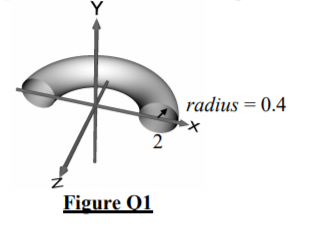
\includegraphics[width=6cm]{fig/q1.PNG}
        \centering
    \end{figure}

    Therefore, it is a \textbf{trapezium}.

\end{homeworkProblem}
\pagebreak
\begin{homeworkProblem}
    Figure Q2 shows a 2D house model and a 2D affine transformation matrix $\mathbf{M}$.
    \begin{enumerate}[i]
        \item Apply $\mathbf{M}$ to the house and sketch the transformed model. Label the
        coordinates of all vertices on your sketched figure.
        \item This matrix  $\mathbf{M}$ represents a composition of several basic transformations.
        Write the matrix for each basic transformation and describe the order of these transformations.
        Note that translation, rotation and scaling are basic transformations.
    \end{enumerate}
    
    \begin{figure}[H]
        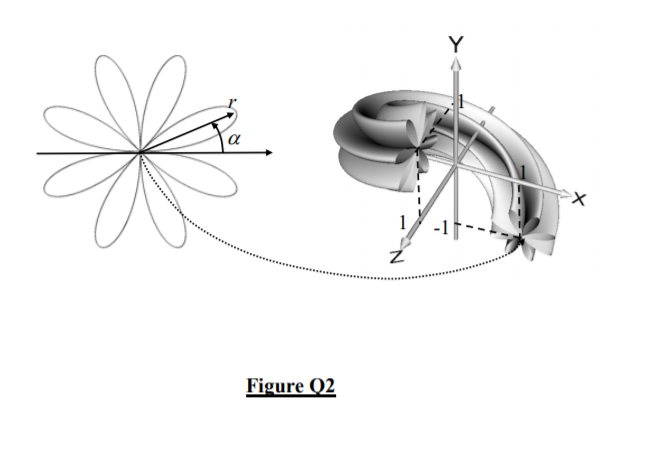
\includegraphics[width=8cm]{fig/q2.PNG}
        \centering
    \end{figure}

    \textbf{Solution}\\
    \textbf{Part i:}
    First, we label the vertices on the original figure and obtain their homogenous coordinates:
    \begin{figure}[H]
        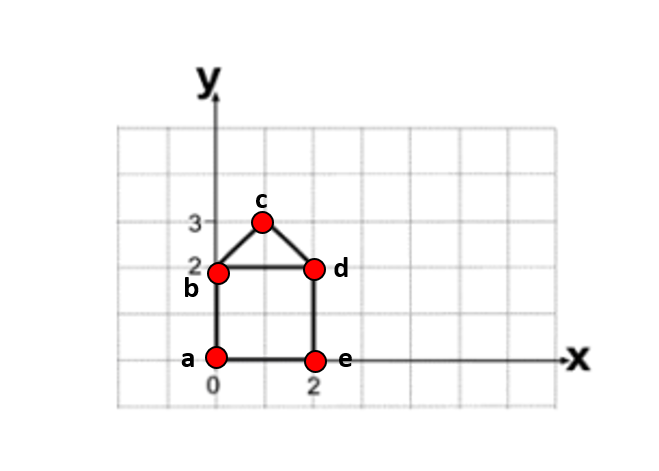
\includegraphics[width=7cm]{fig/q2a.PNG}
        \centering
    \end{figure}
    $a = \begin{bmatrix}
            0 \\
            0 \\
            1
         \end{bmatrix}\ b = \begin{bmatrix}
        0 \\
        2 \\
        1
     \end{bmatrix}\ c= \begin{bmatrix}
        1 \\
        3 \\
        1
     \end{bmatrix}\ d= \begin{bmatrix}
        2 \\
        2 \\
        1
     \end{bmatrix}\ e= \begin{bmatrix}
        2 \\
        0 \\
        1
     \end{bmatrix} $\\\\
    Multiplying $\mathbf{M}$ to all vertices,\\
    $a = \begin{bmatrix}
        0 & -0.5 & 0.5 \\
        2 & 0 & 2 \\
        0 & 0 & 1
     \end{bmatrix}\begin{bmatrix}
        0 \\
        0 \\
        1
     \end{bmatrix}=\begin{bmatrix}
        0.5 \\
        2 \\
        1
     \end{bmatrix}\ b = \begin{bmatrix}
        0 & -0.5 & 0.5 \\
        2 & 0 & 2 \\
        0 & 0 & 1
     \end{bmatrix}\begin{bmatrix}
    0 \\
    2 \\
    1
 \end{bmatrix}=\begin{bmatrix}
    -0.5 \\
    2 \\
    1
 \end{bmatrix}\\c= \begin{bmatrix}
    0 & -0.5 & 0.5 \\
    2 & 0 & 2 \\
    0 & 0 & 1
 \end{bmatrix}\begin{bmatrix}
    1 \\
    3 \\
    1
 \end{bmatrix}=\begin{bmatrix}
    -1 \\
    4 \\
    1
 \end{bmatrix}\ d= \begin{bmatrix}
    0 & -0.5 & 0.5 \\
    2 & 0 & 2 \\
    0 & 0 & 1
 \end{bmatrix}\begin{bmatrix}
    2 \\
    2 \\
    1
 \end{bmatrix}=\begin{bmatrix}
    -0.5 \\
    6 \\
    1
 \end{bmatrix}\\e= \begin{bmatrix}
    0 & -0.5 & 0.5 \\
    2 & 0 & 2 \\
    0 & 0 & 1
 \end{bmatrix}\begin{bmatrix}
    2 \\
    0 \\
    1
 \end{bmatrix} =\begin{bmatrix}
    0.5 \\
    6 \\
    1
 \end{bmatrix}$

Sketching the resulting house using the new locations of the vertices, we get the following:
\begin{figure}[H]
    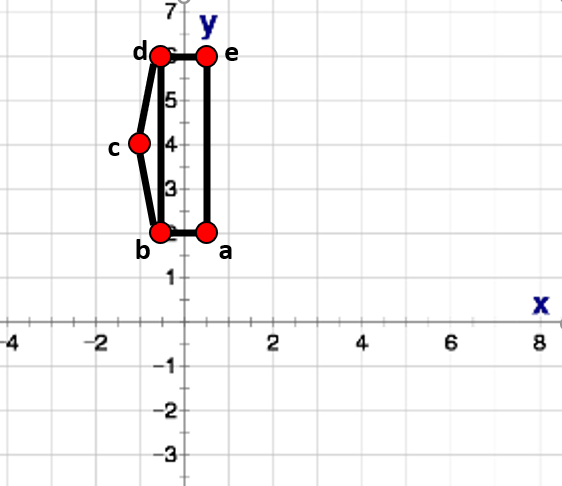
\includegraphics[width=7cm]{fig/q2b.PNG}
    \centering
\end{figure}

\textbf{Part ii:}
We can visually deduce the basic transformations and the order they were performed:
\begin{enumerate}
    \item Rotate CCW about origin for 90 degrees / $0.5\pi$ 
    \item Scale in Y axis by 2 times, X axis by 0.5 times.
    \item Translate by y: +2, x: +0.5
\end{enumerate}
We get the matrices for the basic transformations described above,\\
$R = \begin{bmatrix}
    cos(0.5\pi) & -sin(0.5\pi) & 0 \\
    sin(0.5\pi) & cos(0.5\pi) & 0 \\
    0 & 0 & 1
 \end{bmatrix} = \begin{bmatrix}
    0 & -1 & 0 \\
    1 & 0 & 0 \\
    0 & 0 & 1
 \end{bmatrix}$\\
 $S = \begin{bmatrix}
    0.5 & 0 & 0 \\
    0 & 2 & 0 \\
    0 & 0 & 1
 \end{bmatrix}$\\
 $T = \begin{bmatrix}
    1 & 0 & 0.5 \\
    0 & 1 & 2 \\
    0 & 0 & 1
 \end{bmatrix}$\\
 Now we try to apply the transformation matrices in reverse order (i.e., TSR):\\
 $SR = \begin{bmatrix}
    0.5 & 0 & 0 \\
    0 & 2 & 0 \\
    0 & 0 & 1
 \end{bmatrix}\begin{bmatrix}
    0 & -1 & 0 \\
    1 & 0 & 0 \\
    0 & 0 & 1
 \end{bmatrix} = 
 \begin{bmatrix}
    0 & -0.5 & 0 \\
    2 & 0 & 0 \\
    0 & 0 & 1
 \end{bmatrix}$\\

 $TSR = \begin{bmatrix}
    1 & 0 & 0.5 \\
    0 & 1 & 2 \\
    0 & 0 & 1
 \end{bmatrix}\begin{bmatrix}
    0 & -0.5 & 0 \\
    2 & 0 & 0 \\
    0 & 0 & 1
 \end{bmatrix} = 
 \begin{bmatrix}
    0 & -0.5 & 0.5 \\
    2 & 0 & 2 \\
    0 & 0 & 1
 \end{bmatrix} = \mathbf{M}$\\

 As we see that the resultant affine matrix is the same as \textbf{M}, we conclude that 
 the transformation matrices and the order they are applied are correct.
    
\end{homeworkProblem}

\pagebreak
\begin{homeworkProblem}
    A 2D geometric object is scaled with respect to the point with coordinates $(1,1)$
    in the x-coordinate by 5 times and the y-coordinate by 3 times. Then the object is 
    rotated about the origin by $90^\circ$ in the clockwise direction. Finally, the object 
    is reflected through the x-axis. Write in a proper order the matrices constituting this 
    transformation.\\\\
    \textbf{Solution}\\
    Steps:
    \begin{enumerate}
        \item Translate by x: -1, y:-1 ($\mathbf{T_1}$)
        \item Scale by: x: 5, y:3 ($\mathbf{S_1}$)
        \item Translate by x: 1, y: 1 ($\mathbf{T_2}$)
        \item Rotate by $90^\circ$ clockwise ($\mathbf{R_1}$)
        \item Reflect by x-axis ($\mathbf{R_2}$)
    \end{enumerate}

    Proper order of multiplying matrices for the transformation:
    $X' = R_2R_1T_2S_1T_1 X$


\end{homeworkProblem}

\pagebreak
\begin{homeworkProblem}
    Let $\mathbf{R}$ be a 2D rotation about the origin and $\mathbf{T}$ a 2D translation.
    Do $\mathbf{RT}$ and $\mathbf{TR}$ define the same composite transformation? Justify
    your answer mathematically\\\\

    \textbf{Solution}\\
    For rotation,\\
    $R = \begin{bmatrix}
        cos(\alpha) & -sin(\alpha) & 0 \\
        sin(\alpha) & cos(\alpha) & 0 \\
        0 & 0 & 1
    \end{bmatrix}$\\
    Let $a = cos(\alpha)$, $b = sin(\alpha)$\\
    $R = \begin{bmatrix}
        a & -b & 0 \\
        b & a & 0 \\
        0 & 0 & 1
    \end{bmatrix}$
    \\\\
    For translation,\\
    $T = \begin{bmatrix}
        1 & 0 & t_x \\
        0 & 1 & t_y \\
        0 & 0 & 1
    \end{bmatrix}$\\\\
    Therefore,
    \\
    $RT = \begin{bmatrix}
        a & -b & 0 \\
        b & a & 0 \\
        0 & 0 & 1
    \end{bmatrix}\begin{bmatrix}
        1 & 0 & t_x \\
        0 & 1 & t_y \\
        0 & 0 & 1
    \end{bmatrix} = 
    \begin{bmatrix}
        a & -b & at_x - bt_y + 1\\
        b & a & bt_x + at_y + 1\\
        0 & 0 & 1
    \end{bmatrix}$\\\\


    $TR = \begin{bmatrix}
        1 & 0 & t_x \\
        0 & 1 & t_y \\
        0 & 0 & 1
    \end{bmatrix}\begin{bmatrix}
        a & -b & 0 \\
        b & a & 0 \\
        0 & 0 & 1
    \end{bmatrix} = 
    \begin{bmatrix}
        a & -b & t_x \\
        b & a & t_y \\
        0 & 0 & 1
    \end{bmatrix}$\\\\

    Hence, RT and TR do not define the same transformations.
\end{homeworkProblem}

\end{document}